\documentclass[paper=a4]{article}
\usepackage{ucs}
\usepackage[utf8x]{inputenc}
\usepackage[T1]{fontenc}
\PreloadUnicodePage{0}
\usepackage{xspace}
\usepackage{array}
\usepackage[hmargin=3.5cm,vmargin=2.7cm]{geometry} 
\usepackage{graphicx}



\begin{document}
\title{ \normalsize 
\includegraphics[scale=0.43]{images/CarGameLogo.png}
	\\
	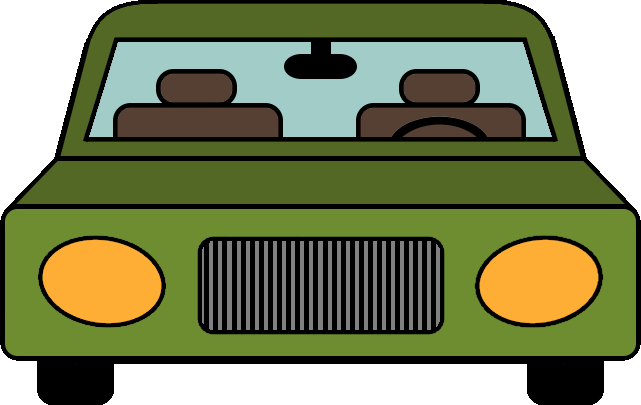
\includegraphics[scale=0.5]{images/menu_car.png}
}
\author{Team Dank \\
Universitetet i Bergern \\
Informatikk}
\maketitle
\newpage

\section{Introduksjon}
Dette er et spill tiltenkt datamaskiner der spilleren kjører en bil.
Bilen kjører langs en vei med forskjellige ting i veibanen, som spilleren kan kjøre over eller unngå.
Vanndammer vil gjøre at spilleren mister drivstoff, og mister litt kontrollen over bilen.
Kumlokk i veien gjør at spilleren taper.
Bensintanker gir spilleren ekstra drivstoff, slik at runden varer lenger.
Myke trafikanter vil gi poeng til spilleren dersom de blir påkjørt.
Mynter kan plukkes opp slik at spilleren kan kjøpe nye biler.
Spilleren får en score for hver spillrunde, i tillegg til at spilleren samler opp virtuelle penger som kan brukes til å bytte bil.
\newpage

\section{Systemkrav og installasjon}
\subsection{Systemkrav}
\begin{itemize}
	\item Ikke mindre enn 1 GB RAM minne\\
	\item Windows Vista/Linux 2005/Mac OS X eller senere \\
	\item 50 MB ledig plass for installasjon \\
	\item Java 8 \\
	\item Tastatur, mus \\
 	\item TeamDank anbefaler deg å ha en prosessor (2005+) med \\ 
klokkefrekvens på 1.6 Ghz eller bedre.
\end{itemize}
\subsection{Installasjon}
Du må først sørge for at du har installert den nyeste versjonen av Java og \\
for å kunne spille Carl the Crasher må du laste ned carlthecrasher.jar filen. \\
Deretter åpner du filen som vanlig for å starte spillet.   
\newpage

\section{Spillinstruksjoner og -regler} 
Som Carl liker du å kjøre uforsvarlig, og målet ditt er å komme deg så lengst mulig uten gå tom for bensin og få mest mulig poeng. \\
Din primære spillinngangsenhet er tastaturen, og kan gjøre følgende: 
\begin{itemize}
	\item Du styrer Carl til høyre og venstre ved å bruke enten piltastene eller tastaturknappene \\ A og D. \\ 
	\item Carl kan ikke styre bilens hastighet direkte, men farten vil økes jo lenger du kjøre.
	\item Du kan ikke kjøre ut av veien, men du kan kjøre på objekter som oppstår på veien.
	\item Du kan pause spillet ved å gå til pausemenyen ved å trykke på tastaturknappen ESC. 
	\begin{itemize}
		\item Å trykke på ESC vil gi deg muligheten til å fortsette eller avsluttet spillet.
	\end{itemize}
\end{itemize}
På veien kan det oppstå forskjellige objekter, og avhengig av objektet kan det påføre bilen en positiv, eller negativ effekt. \\
\begin{itemize}
	\item 
\includegraphics[scale=0.2]{images/gastank.png} Bensintank: Kan plukkes for å øke drivstoffen slik at du kan kjøre lengre 
	\item 
\includegraphics[scale=0.5]{images/coin.png} Mynt: På veien kan du finne mynter som du kan plukke opp.5
																Myntene kan brukes i butikken for å kjøpe nye biler.
	\item 
\includegraphics[scale=0.2]{images/puddle.png} Vanndam: Kjører du på en vanndam vil det minske mengden drivstoff,
																og samtidig gjøre at du vil miste litt kontrollen av bilen i en liten periode. 
	\item 
\includegraphics[scale=0.2]{images/manhole.png} Kumlokk: Dersom du kjører på en kumlokk vil du kræsje og deretter tape umiddelbart
	\item 
\includegraphics[scale=0.4]{images/walker.png} Myke trafikanter: Å kjøre på trafikanter vil gi deg ekstra poeng som vil øke sluttpoengsummen din 
\end{itemize}
\newpage

\begin{center}
\begin{tabular}{ | m{5cm} | m{8cm} | }
\hline
Målgruppe. & Ungdom 15-25 år. \\ \hline



Åpne data. & Bruke åpne data fra yr.no om været. Om det er skyer vil det være skyer på banen,\\&
om det regner vil det regne på banen, og om det snør vil det være snø på banen.\\ \hline
\end{tabular}
\end{center}

		\subsection{Poeng}
		\begin{itemize}
			\item{Spilleren tjener poeng konstant når han kjører.}
			\item{Poeng blir opptjent avhengig av hvor langt spilleren kjører og hvilke myke trafikanter spilleren kjører over.}
			\item{Spilleren starter alltid med 0 poeng i starten av en runde.}
		\end{itemize}

		\subsection{Penger}
		\begin{itemize}
			\item{I løpet av spillet får spilleren penger i form av spillets egen valuta.}
			\item{Pengene kan brukes i spillets butikk fra hovedmenyen for å kjøpe nye biler.}
		\end{itemize}

	\newpage
	\begin{figure}\begin{center}
		
\includegraphics[width=1.00\textwidth]{images/main_menu.PNG}
		\caption{Hovedmeny.}
	\end{center}\end{figure}

	\begin{figure}\begin{center}
		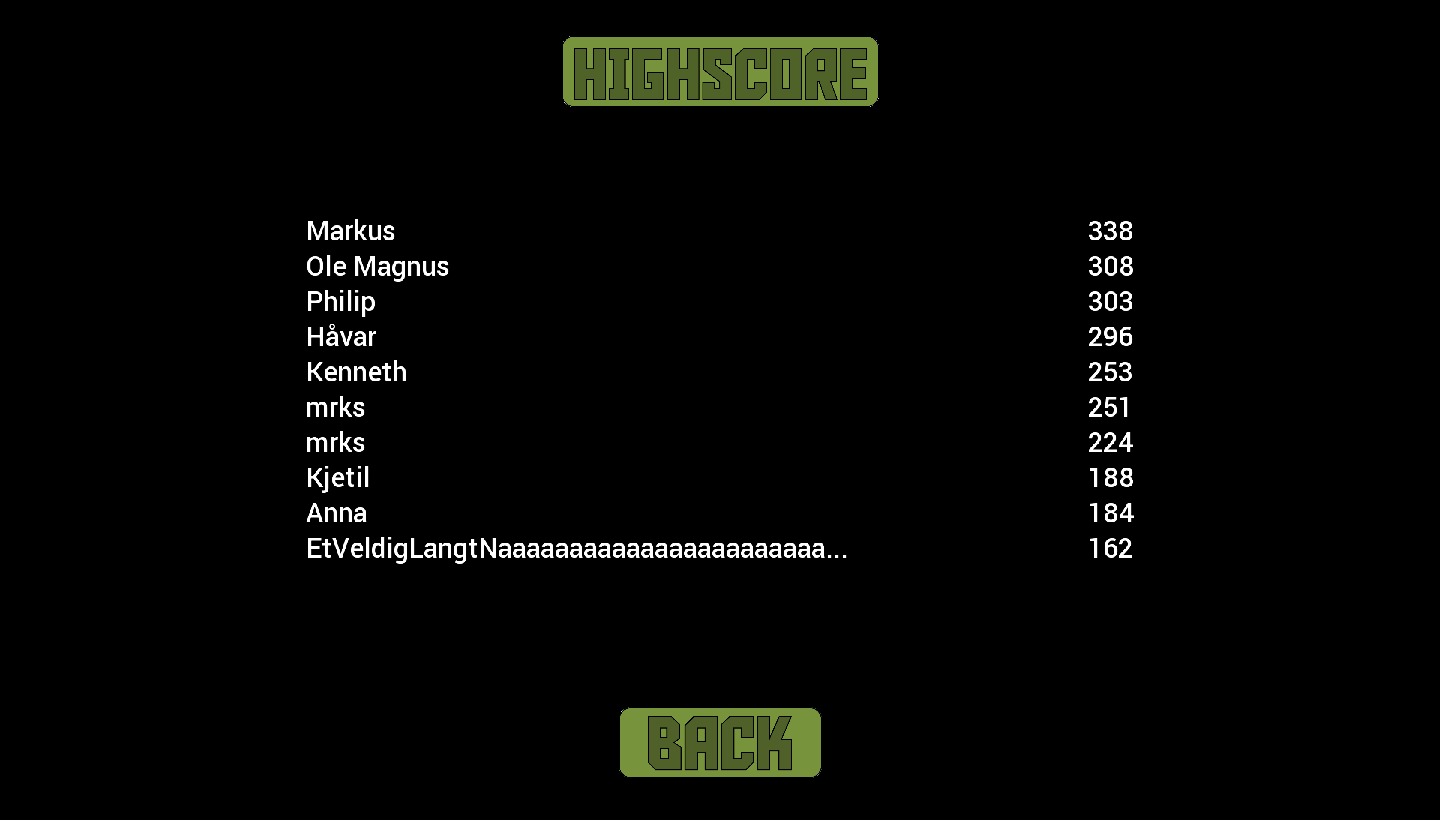
\includegraphics[width=1.00\textwidth]{images/hs_menu.PNG}
		\caption{Highscoremeny.}
	\end{center}\end{figure}

	\begin{figure}\begin{center}
		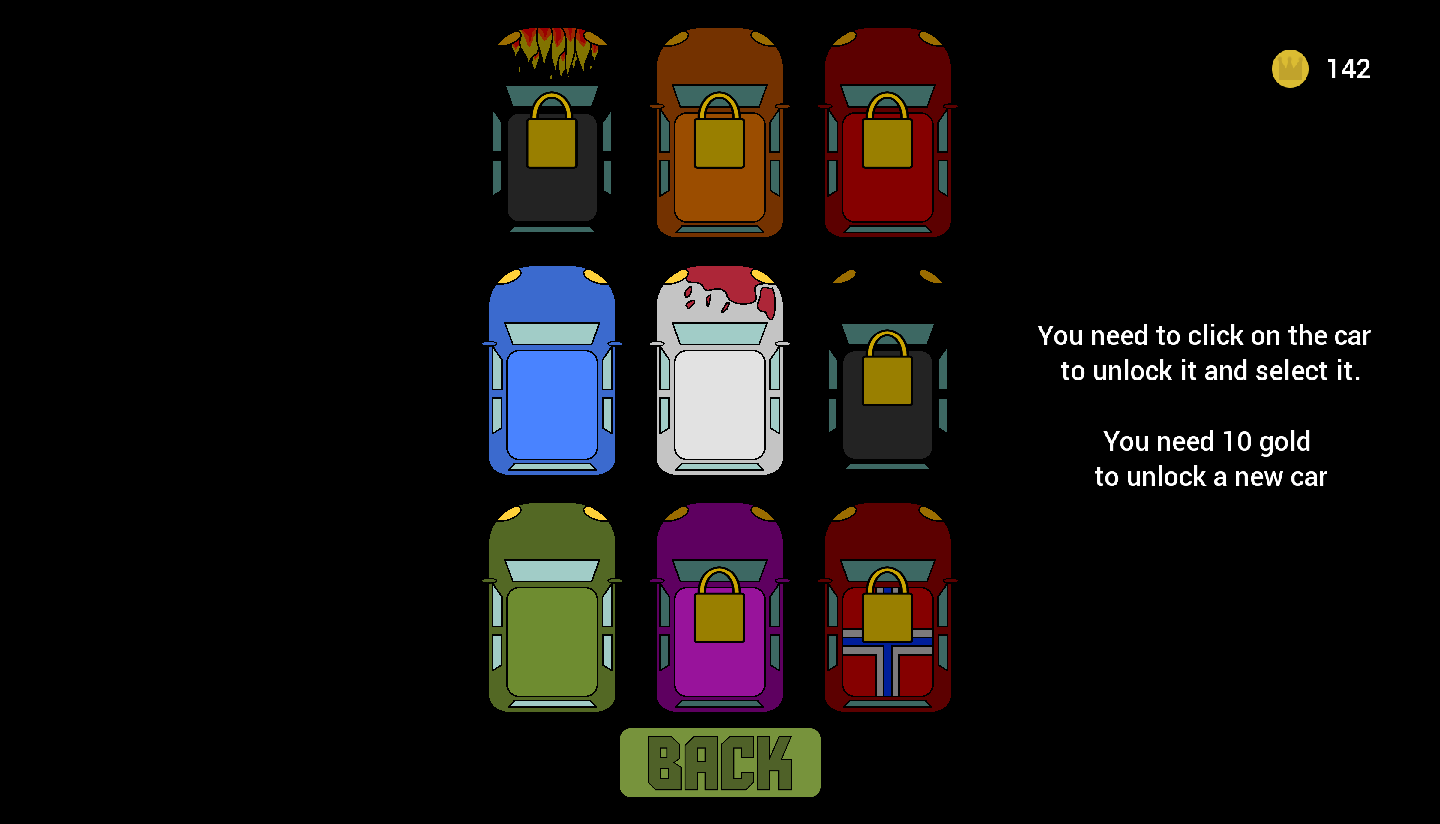
\includegraphics[width=1.00\textwidth]{images/shop_menu.PNG}
		\caption{Butikkmeny.}
	\end{center}\end{figure}

	\begin{figure}\begin{center}
		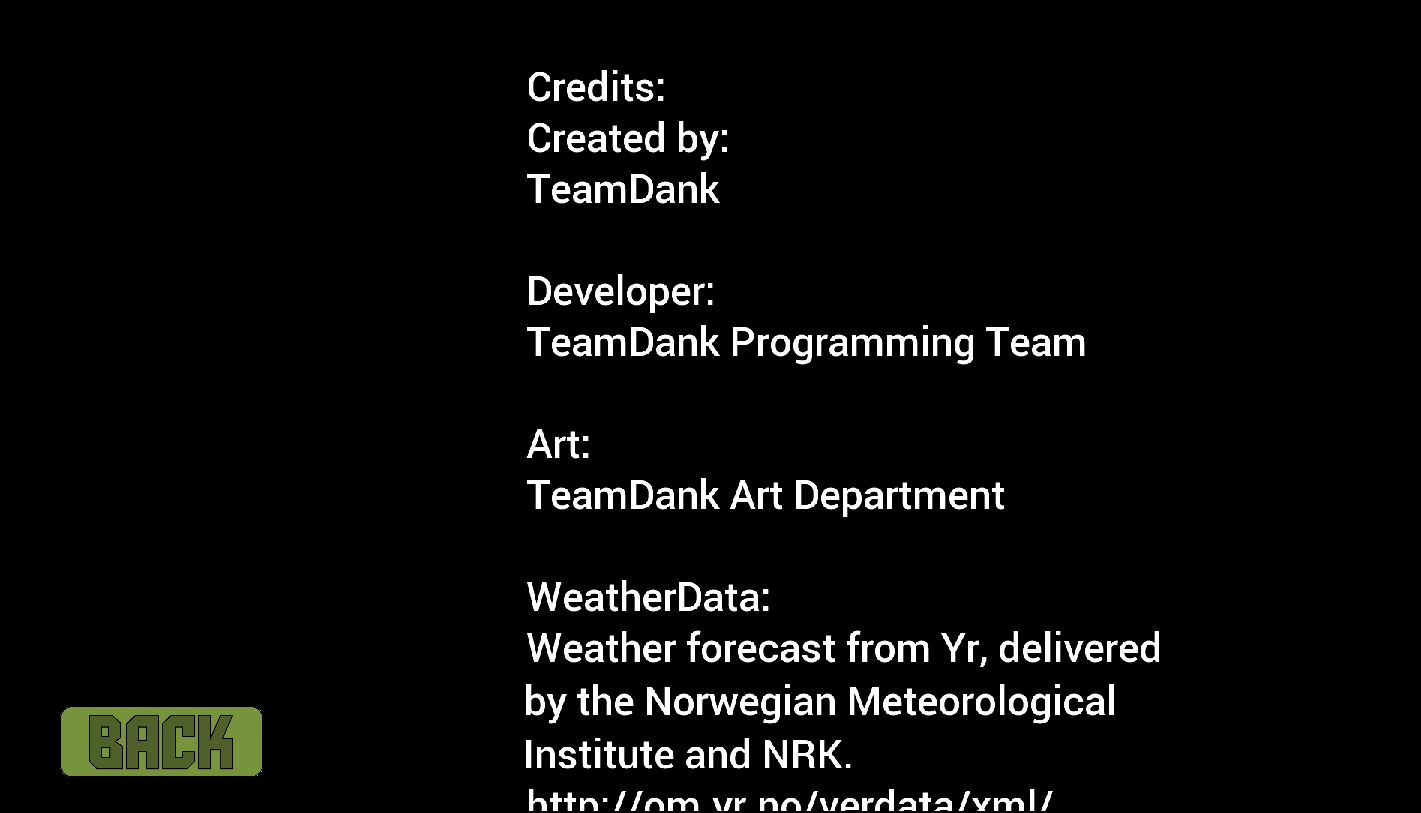
\includegraphics[width=1.00\textwidth]{images/credits.PNG}
		\caption{Kreditering.}
	\end{center}\end{figure}

	\begin{figure}\begin{center}
		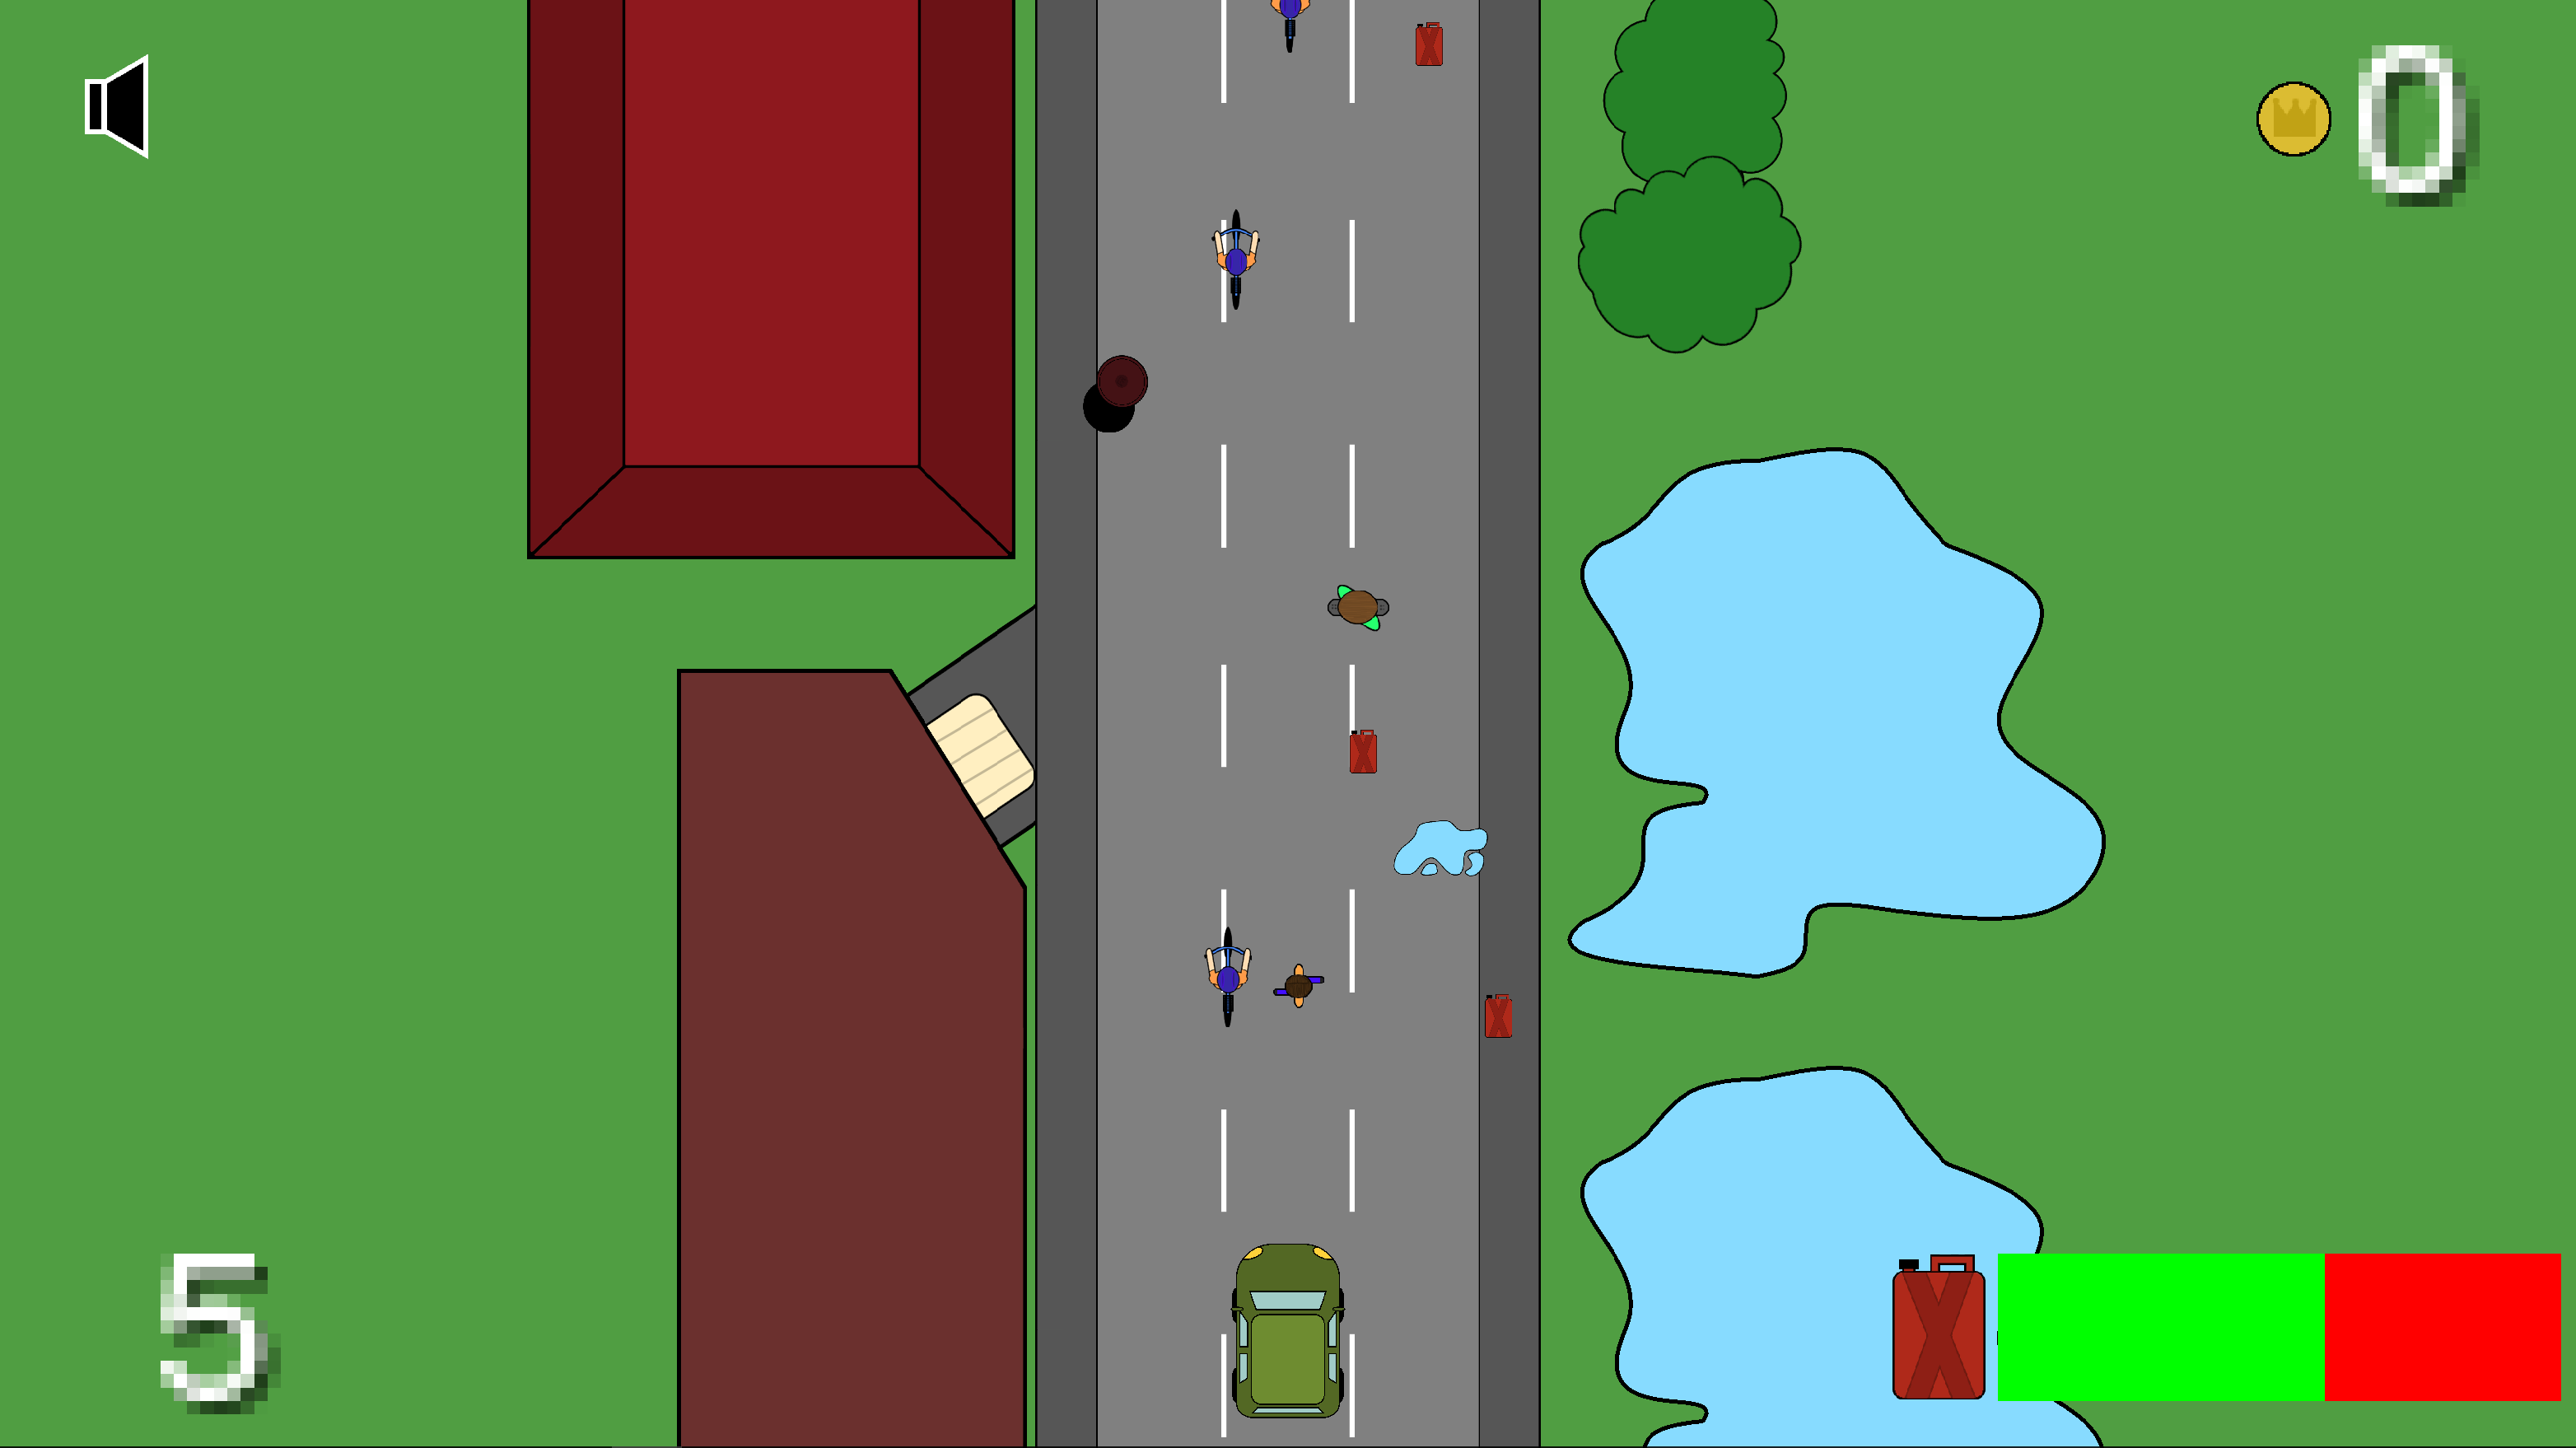
\includegraphics[width=1.00\textwidth]{images/game.PNG}
		\caption{Gameplay.}
	\end{center}\end{figure}

	\begin{figure}\begin{center}
		
\includegraphics[width=1.00\textwidth]{images/pause.PNG}
		\caption{Pausemeny.}
	\end{center}\end{figure}

	\begin{figure}\begin{center}
		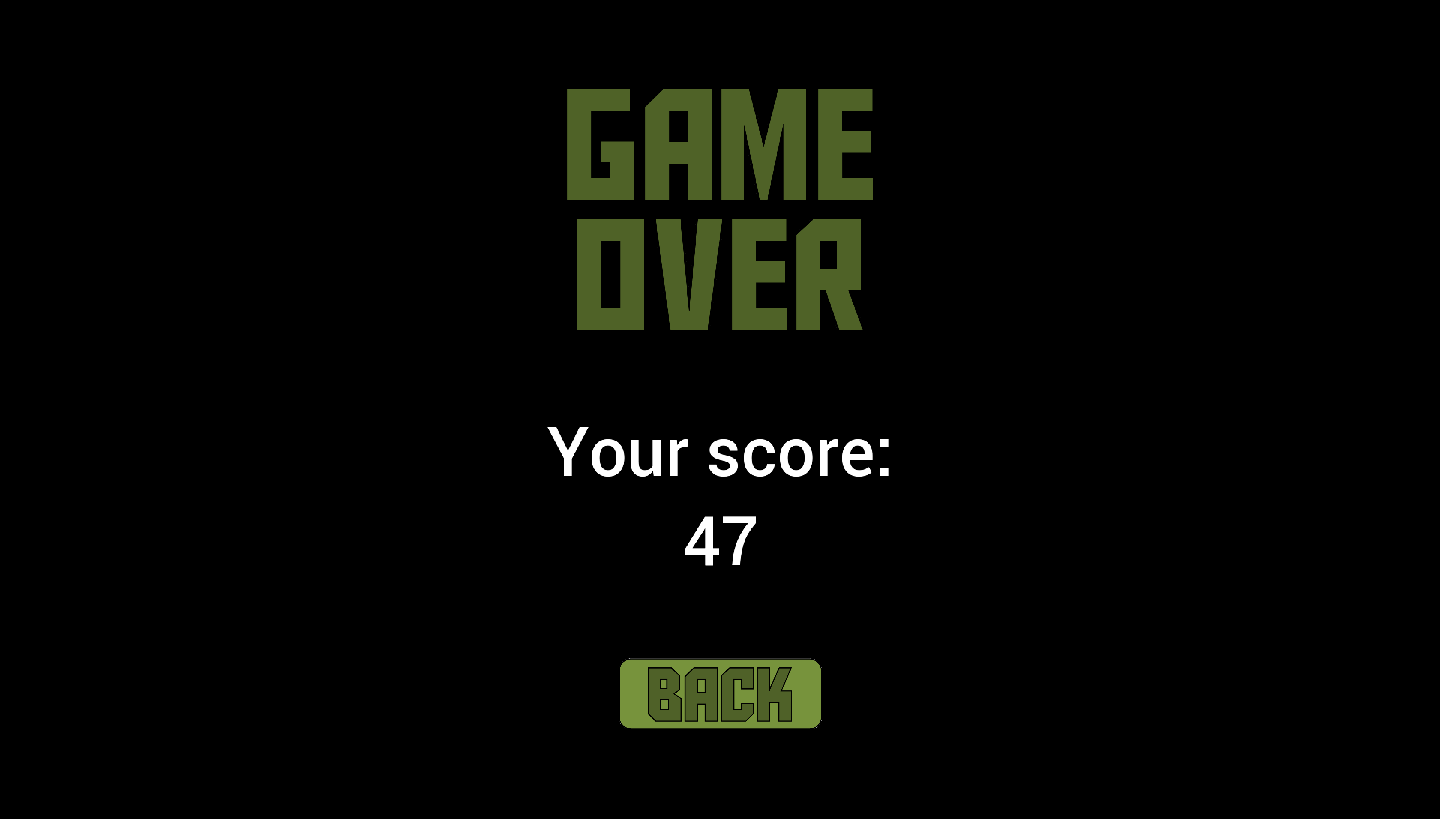
\includegraphics[width=1.00\textwidth]{images/gameover.PNG}
		\caption{Game over-meny.}
	\end{center}\end{figure}


\end{document}